\documentclass[pdflatex,lib/sn-mathphys-num]{lib/sn-jnl}% Math and Physical Sciences Numbered Reference Style

% \documentclass[pdflatex,sn-mathphys-num]{sn-jnl}% Math and Physical Sciences Numbered Reference Style
%%\documentclass[pdflatex,sn-mathphys-ay]{sn-jnl}% Math and Physical Sciences Author Year Reference Style
%%\documentclass[pdflatex,sn-aps]{sn-jnl}% American Physical Society (APS) Reference Style
%%\documentclass[pdflatex,sn-vancouver-num]{sn-jnl}% Vancouver Numbered Reference Style
%%\documentclass[pdflatex,sn-vancouver-ay]{sn-jnl}% Vancouver Author Year Reference Style
%%\documentclass[pdflatex,sn-apa]{sn-jnl}% APA Reference Style
%%\documentclass[pdflatex,sn-chicago]{sn-jnl}% Chicago-based Humanities Reference Style

%%%% Standard Packages
%%<additional latex packages if required can be included here>

\usepackage{graphicx}%
\usepackage{multirow}%
\usepackage{amsmath,amssymb,amsfonts}%
\usepackage{amsthm}%
\usepackage{mathrsfs}%
\usepackage[title]{appendix}%
\usepackage{xcolor}%
\usepackage{textcomp}%
\usepackage{manyfoot}%
\usepackage{booktabs}%
\usepackage{algorithm}%
\usepackage{algorithmicx}%
\usepackage{algpseudocode}%
\usepackage{listings}%
\usepackage{tikz-cd}
\usepackage{ulem}
\usepackage{caption}

\usetikzlibrary{arrows.meta,positioning,fit,backgrounds,calc,decorations.pathreplacing}

%%%%%=============================================================================%%%%
%%%%  Remarks: This template is provided to aid authors with the preparation
%%%%  of original research articles intended for submission to journals published 
%%%%  by Springer Nature. The guidance has been prepared in partnership with 
%%%%  production teams to conform to Springer Nature technical requirements. 
%%%%  Editorial and presentation requirements differ among journal portfolios and 
%%%%  research disciplines. You may find sections in this template are irrelevant 
%%%%  to your work and are empowered to omit any such section if allowed by the 
%%%%  journal you intend to submit to. The submission guidelines and policies 
%%%%  of the journal take precedence. A detailed User Manual is available in the 
%%%%  template package for technical guidance.
%%%%%=============================================================================%%%%

%% as per the requirement new theorem styles can be included as shown below
\theoremstyle{thmstyleone}%
\newtheorem{theorem}{Theorem}%  meant for continuous numbers
%%\newtheorem{theorem}{Theorem}[section]% meant for sectionwise numbers
%% optional argument [theorem] produces theorem numbering sequence instead of independent numbers for Proposition
\newtheorem{proposition}[theorem]{Proposition}% 
%%\newtheorem{proposition}{Proposition}% to get separate numbers for theorem and proposition etc.

\theoremstyle{thmstyletwo}%
\newtheorem{example}{Example}%
\newtheorem{remark}{Remark}%

\theoremstyle{thmstylethree}%
\newtheorem{definition}{Definition}%

\raggedbottom
%%\unnumbered% uncomment this for unnumbered level heads

%%==================================%%
%% Commands                         %%
%%==================================%%
\newcommand{\TODO}[1]{\textcolor{red}{(TODO: #1)}}
\newcommand{\Haotian}[1]{\textcolor{teal}{(Haotian: #1)}}

\newcommand{\logten}[0]{$\log_{10}(n)$}
\newcommand{\sqrtf}[0]{$\sqrt n/5$}
\newcommand{\piecewise}[0]{\texttt{piecewise}}

\newcommand{\figtitle}[1]{{\fontsize{9}{10}\selectfont\bfseries #1}}
\newcommand{\fignote}[1]{{\fontsize{8}{9}\selectfont\color{black!65}#1}}

\newcommand{\hyves}[0]{Hyves}
\newcommand{\orkut}[0]{Orkut}
\newcommand{\livejournal}[0]{Livejournal}
\newcommand{\CEN}[0]{CEN}
\newcommand{\twittersocial}[0]{Twitter\_social}
\newcommand{\OC}[0]{OCv1}
%%==================================%%

\begin{document}

\title[Article Title]{Supplementary Material for DistCM-IL: A post-clustering tool for improved edge-connectivity}

\author[1]{\fnm{Haotian} \sur{Yi}}\email{yi54@illinois.edu}
%\equalcont{These authors contributed equally to this work.}

\author[1]{\fnm{Charles} \sur{Cooper}}\email{ccoop4@illinois.edu}

\author[1]{\fnm{Minhyuk} \sur{Park}}\email{minhyuk2illinois.edu}

\author*[1]{\fnm{Tandy} \sur{Warnow}}\email{warnow@illinois.edu}

\author*[1]{\fnm{George} \sur{Chacko}}\email{chackoge@illinois.edu}
%\equalcont{These authors contributed equally to this work.}


\affil[1]{\orgdiv{Siebel School of Computing and Data Science}, \orgname{The University of Illinois Urbana-Champaign}, \orgaddress{\street{201 N. Goodwin Ave}, \city{Urbana}, \postcode{61801}, \state{Illinois}, \country{USA}}}

\maketitle

% \section{Motivation}
% \subsection{Community Detection}
% Community detection has been studied extensively through a wide range of methodologies~\cite{jin2021surveycommunitydetectionapproaches, huang_survey_2021}. Modularity-based methods, introduced by Newman and Girvan~\cite{newman_girvan_2004} and extended by Newman~\cite{newman2006modularity}, favor clusters with more internal edges than expected from a random null model. The Louvain algorithm~\cite{Blondel_2008} made modularity maximization practical at scale but could produce internally disconnected communities, which the Leiden algorithm~\cite{DBLP:journals/corr/abs-1810-08473} resolves by adding a refinement phase. Leiden also supports using the Constant Potts Model (CPM)~\cite{traag_2011} as the objective, for which any cut that splits a cluster of an optimal clustering into parts $A$ and $B$ has at least $r|A||B|$ size, where $r$ is the resolution parameter. This bound, however, can still be weak in practice~\cite{park_well-connectedness_2024}. Stochastic block models (SBMs)~\cite{holland_1983, karrer_2011, peixoto_2019} instead fit a generative model in which edge probabilities depend on block membership, and can likewise return poorly connected or even disconnected clusters~\cite{park_well-connectedness_2024, vule2025usingstochasticblockmodels}. Flow-based methods such as Infomap~\cite{rosvall_2008} identify communities as groups of nodes that retain a random walker, cut-based methods such as spectral clustering~\cite{shi_malik_2000} and multilevel partitioning~\cite{karypis_1998} seek partitions with small normalized or balanced edge cuts, and deep-learning approaches~\cite{tsitsulin_2023, bianchi_2020} train graph neural networks on relaxed modularity or cut objectives. These methods differ in what they guarantee about cluster connectivity. Many objectives impose no bound on the minimum cut; methods like Leiden under CPM, normalized cut, and Highly Connected Subgraphs~\cite{hartuv_2000} provide connectivity guarantee relative to the resolution parameter or to cluster size and volume. Post-processing methods such as WCC and CM are complementary to all these methods by enforcing a chosen connectivity criterion on the output of any clustering method, whether or not the method carries a guarantee of its own.

\section{DistCM-IL Design \& Implementation Details}
This section describes some additional design and implementation details of  DistCM-IL.

\subsection{Partitioning and Batching} \label{sec:batching}
% \Haotian{One or two sentences with the table.}

Before execution, DistCM-IL makes a sequential pass over the input that partitions the network into self-contained jobs on the shared file system, so that each worker loads only the clusters it processes. With one job per cluster, a clustering with millions of small clusters pays a file-creation cost in this pass, and a head-worker round trip during execution, for every cluster. DistCM-IL therefore groups small clusters into a single job until their combined estimated cost $Y(c)$ reaches a user-specified threshold, which we call a batch. The batch is then stored, assigned, and processed as a unit.

Table~\ref{tab:partition-batch-size} shows the effect on OCv1. Enabling batching at a threshold of 1,000 reduces partitioning time by $1.7\times$ to $7.8\times$, with the largest gain for the clustering with the most clusters. Raising the threshold further changes partitioning time by 10-22\%, in no consistent direction, while leaving the head node fewer and coarser jobs to balance. We therefore set the default threshold to 1,000.

\begin{table}[ht]
    \centering
    \captionsetup{width=\linewidth}
    \caption{\textbf{Effect of batching on Dist-CM partitioning} - Results are taken from network OCv1. Without batching (``None''), every cluster is its own job, so the number of batches equals the number of input clusters. Runtimes and batch counts are means over 3 replicates. Singleton clusters are excluded.}
    \label{tab:partition-batch-size}
    \begin{tabular}{@{}l rr rr rr@{}}
    \toprule
    & \multicolumn{2}{c}{Leiden-Mod}
    & \multicolumn{2}{c}{Leiden-CPM(0.001)}
    & \multicolumn{2}{c@{}}{Leiden-CPM(0.01)} \\
    \cmidrule(lr){2-3} \cmidrule(lr){4-5} \cmidrule(l){6-7}
    Min.\ batch cost & Time (s) & Batches & Time (s) & Batches & Time (s) & Batches \\
    \midrule
    None      & 1{,}147.3 & 183{,}432 & 1{,}803.3 & 840{,}737 & 3{,}710.3 & 2{,}133{,}756 \\
    1{,}000   & 675.0     & 1{,}469   & 514.0     & 88{,}939  & 473.3     & 149{,}153 \\
    10{,}000  & 674.3     & 195       & 625.7     & 14{,}265  & 389.3     & 16{,}349 \\
    100{,}000 & 604.0     & 67        & 609.7     & 1{,}557   & 374.3     & 1{,}653 \\
    \bottomrule
    \end{tabular}
\end{table}

\subsection{Work Sharing} \label{sec:work-sharing}
To avoid a large cluster from bottlenecking a worker, DistCM-IL allows subsequent tasks to be shared with other workers as the cluster is decomposed. When a CM iteration produces more than one sub-cluster above a user-specified size threshold, the worker keeps the largest and yields the others to the head node, which inserts them into its priority queue like other assignable jobs. Sub-clusters smaller than the threshold are kept locally to reduce communication overhead. The mechanism is recursive in nature: a worker that receives a shared sub-cluster may further share parts of it, so a large cluster fans out into a tree of progressively smaller jobs spread across many workers (Figure.~\ref{fig:work-redistribution}).

Since work is now split across this tree, completion must be tracked hierarchically. The head node marks a cluster complete only once every sub-cluster yielded from it has completed. Only then is every node of the original cluster guaranteed to have been processed by the post-processing algorithm and counted toward overall progress.

Yielding a sub-cluster requires writing its edgelist to the shared file system and reading it back on another worker, so each redistribution incurs I/O proportional to the sub-cluster's size. The threshold therefore controls a trade-off: a low threshold redistributes aggressively, maximizing parallelism but multiplying I/O, whereas a high threshold avoids communication at the risk of letting a large cluster to bottleneck a single worker. We use a default of 100,000 nodes, chosen so that the time saved by processing a sub-cluster in parallel outweighs the I/O cost of moving it.

\begin{figure}[t]
  \centering
  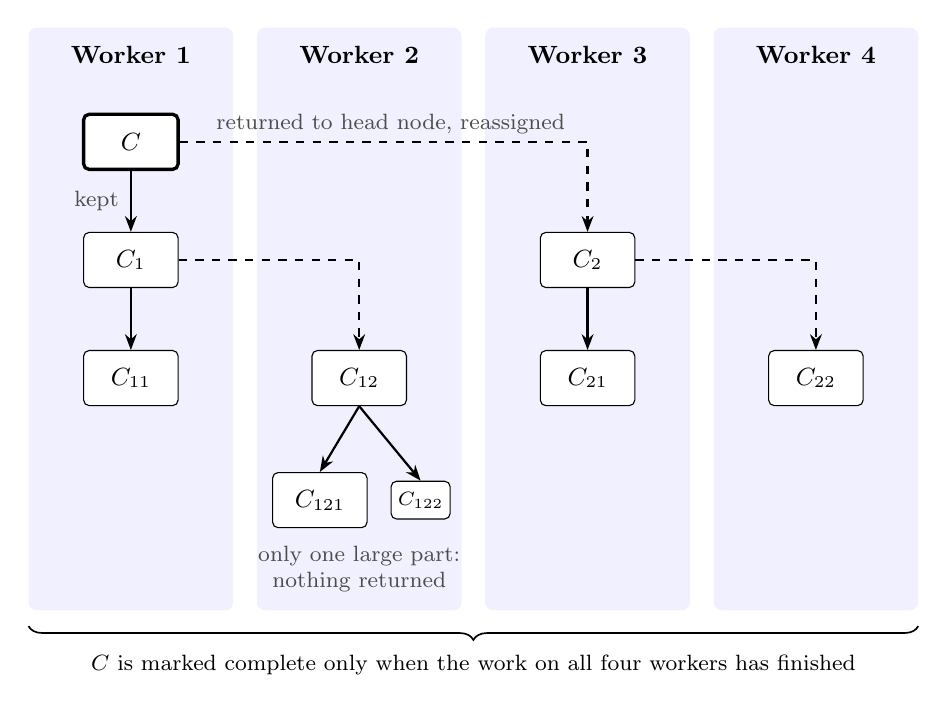
\begin{tikzpicture}[
      font=\small,
      lane/.style={fill=blue!6, rounded corners=3pt},
      big/.style={draw, rounded corners=2pt, fill=white, minimum width=1.2cm,
                  minimum height=0.7cm, inner sep=2pt},
      small/.style={draw, rounded corners=2pt, fill=white, minimum width=0.75cm,
                    minimum height=0.48cm, inner sep=1pt, font=\scriptsize},
      keep/.style={-{Stealth[length=2mm]}, thick},
      ret/.style={-{Stealth[length=2mm]}, thick, dashed},
      lbl/.style={font=\footnotesize, inner sep=2pt, text=black!70},
  ]
 
  % ---- One lane per worker ---------------------------------------------
  \foreach \i/\x in {1/0, 2/2.9, 3/5.8, 4/8.7} {
      \fill[lane] (\x-1.3, 1.45) rectangle (\x+1.3, -5.95);
      \node[font=\small\bfseries] at (\x, 1.1) {Worker \i};
  }
 
  % ---- Clusters --------------------------------------------------------
  \node[big, very thick] (C)    at (0,    0)    {$C$};
  \node[big]             (C1)   at (0,   -1.5)  {$C_{1}$};
  \node[big]             (C2)   at (5.8, -1.5)  {$C_{2}$};
  \node[big]             (C11)  at (0,   -3.0)  {$C_{11}$};
  \node[big]             (C12)  at (2.9, -3.0)  {$C_{12}$};
  \node[big]             (C21)  at (5.8, -3.0)  {$C_{21}$};
  \node[big]             (C22)  at (8.7, -3.0)  {$C_{22}$};
  \node[big]             (C121) at (2.4, -4.55)  {$C_{121}$};
  \node[small]           (C122) at (3.68, -4.55)  {$C_{122}$};
 
  % ---- Kept: processed on the same worker ------------------------------
  \draw[keep] (C)  -- (C1) node[lbl, midway, left=2pt] {kept};
  \draw[keep] (C1) -- (C11);
  \draw[keep] (C2) -- (C21);
  \draw[keep] (C12.south) -- (C121.north);
  \draw[keep] (C12.south) -- (C122.north);
 
  % ---- Returned to the head node, reassigned to another worker ---------
  \draw[ret] (C.east)  -| (C2.north);
  \node[lbl, anchor=south] at (3.3, 0.02) {returned to head node, reassigned};
  \draw[ret] (C1.east) -| (C12.north);
  \draw[ret] (C2.east) -| (C22.north);
 
  % ---- Local-only split ------------------------------------------------
  \node[lbl, align=center] at (2.9, -5.42) {only one large part:\\nothing returned};
 
  % ---- Hierarchical completion -----------------------------------------
  \draw[decorate, decoration={brace, mirror, amplitude=5pt}, semithick]
      (-1.3, -6.15) -- (10.0, -6.15)
      node[midway, below=7pt, font=\footnotesize]
      {$C$ is marked complete only when the work on all four workers has finished};
 
  \end{tikzpicture}
  \vspace{4pt}% extra space between figure and caption; no \newline needed
  \caption{\textbf{Recursive work sharing} - Each box is a cluster and each column is the worker that processes it. When a split produces more than one sub-cluster above the size threshold, the worker keeps one (solid arrows) and returns the others to the head node, which reassigns them to idle workers (dashed arrows). A reassigned sub-cluster can be split and returned again ($C_2$), whereas a split with only one large part stays on the same worker ($C_{12}$). The head node marks $C$ complete only when all work derived from it has finished. If any part fails, $C$ is marked aborted.}
  \label{fig:work-redistribution}
\end{figure}

\subsection{Termination Logic}\label{appendix:ssec:termination}
After all initial clusters are either completed or aborted, the program enters the termination phase, in which results are aggregated into the final output. Since each assignment produces a self-contained result, the final clustering is constructed by combining the results of each individual cluster. DistCM-IL implements a simplification of this classic reduction process with two levels, where each worker first merges the results of all completed clusters it worked on into a single local output, before the head node merges the outputs of all workers into the final clustering. This two-level scheme could be generalized to a tree-structured reduction with $O(\log N)$ complexity using $N$ workers, but in practice the  termination phase takes negligible time compared to the actual processing, so we keep this simplified implementation.

\subsection{Fault Tolerance}\label{ssec:fault-tolerance}
% \Haotian{Move to appendix; fault-tolerance is a software design, not very relevant to the analysis we will be doing.}

Because the induced subgraphs at each level of recursion are independent, a failure while processing one cluster cannot affect the others. DistCM-IL exploits this independence through a checkpointing mechanism. The system preserves progress and allows execution to quickly resume after individual cluster failures.

Progress is recorded at the granularity of initial clusters. When a cluster fails - whether from timeout, out-of-memory, or other faults - it is marked incomplete and written to the checkpoint file; if any descendant sub-cluster produced from it by work-sharing fails, the entire initial cluster is likewise marked incomplete. On resumption, the head node loads the checkpoint and assigns only the incomplete clusters. This coarse granularity trades some redundant recomputation for simplicity and correctness: it avoids the machinery needed to track and validate the intermediate state of partially completed clusters, which could otherwise leave the system corrupted. Finer-grained checkpointing that recovers partial progress within a cluster is a promising direction for further improving efficiency on extreme-scale networks.

%\bibliography{bib}
%\clearpage
\end{document}